\documentclass{beamer}
\usepackage[spanish]{babel}
\usepackage[utf8]{inputenc}
\usepackage{graphicx}

\title[La bisección de $f(x)=cos($\pi$x)$ en \textsc{Beamer}]{Bisección con $f(x)=cos($\pi$x)$}
\author[D. Montesdeoca y  L. Martín]{Carmen Laura Martín González
y
David Tomás Montesdeoca Flores}
\date[11/05/14]{11 de mayo de 2014}
\usetheme{Madrid}

\definecolor{ColorMorado}{RGB}{122,59,122}
\setbeamercolor*{palette primary}{use=stucture, fg=white, bg=ColorMorado}
\begin{document}

\begin{frame}

\includegraphics[width=0.15\textwidth]{ULL.jpeg}
\hspace*{7.5cm}

\includegraphics[width=0.16\textwidth]{logocentro.jpeg}
\hspace*{7.5cm}
\titlepage
\end{frame}

\begin{frame}
\frametitle{Indice}
\tableofcontents[pausesections]

\end{frame}

\section{Definición de Bisección}

\begin{frame}
\frametitle{Definición de Bisección}

Según la RAE, La bisección es la acción o efecto de bisecar,es decir, dividir a la mitad y se aplica generalmente en la división de ángulos. Aunque esta definición no se aleja mucho de la deseada, la que verdaderamente nos interesa es la siguiente:

\begin{block}{Definición aplicada}
El método de bisección es un algoritmo usado en matemáticas para llevar a cabo una búsqueda de raíces. En resumen, este método encuentra una raíz de $f(x)=0$. Este método se realiza dividiendo el intervalo a la mitad y seleccionando el subintervalo de estos que contiene la raíz, que es aquel en el que hay un cambio de signo.(Se sabe que una raíz esta en un intervalo cerrado si la función cambia de signo en los puntos extremos). Cuantas más cifras decimales queramos obtener más divisiones tendremos que realizar.
\end{block} 

\end{frame}

\section{Definición del número $\pi$}

\begin{frame}
\frametitle{Definición del número $\pi$}
\begin{block}{Definición}
El número $\pi$ es la relación existente entre el diámetro de la circunferencia con su longitud.
Es un número irracional de los más importantes usados en las ciencias matemáticas, como la física, las ingenierías y las propias matemáticas.

El valor que toma esta constante es aproximadamente:
 $$\pi = 3.14159265358979323846...$$
\end{block}
El número $\pi$ se puede calcular mediante integración:

$$\int_{0}^{1} \! \frac{4}{1+x^2}\, dx = 4(atan(1) -atan(0)) = \pi $$

\end{frame}

\section{Ejemplo general de bisección}

\begin{frame}
\frametitle{Ejemplo general de bisección.}

\begin{block}{}
En la figura, se muestra gráficamente como los valores sucesivos convergen en una raíz de $f(x)$ cuando se empiezan con un par de valores que encierran una raíz. Podemos ver que 5.5 está a la mitad entre 4 y 6, y que 5.75 a la mitad entre 5.5 y 6. Siempre se considera al siguiente valor x al punto medio del último par que encierra entre corchetes a la raíz: Estos valores encierran a la raíz cuando $f(x)$ cambia de signo en los dos puntos.
\end{block}

\begin{figure}[b]
\begin{center}
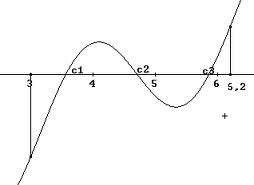
\includegraphics[scale=0.4]{images.jpeg}
\end{center}
\end{figure}

\end{frame}

\section{Teorema de bisección}

\begin{frame}
\frametitle{Teorema de Bisección}
\begin{block}{Teorema}
Si $[a_0, b_0],[a_1,b1],...,[a_n,b_n],...,$ denotan los intervalos en el método de la bisección, entonces los límites $\lim_{n\rightarrow \infty} a_n$ y $\lim_{n\rightarrow \infty}b_n $ existen , son iguales y representan un cero de f. Si r=$\lim_{n\rightarrow \infty}c_n$ y $c_n=(a_n+b_n)$ entonces: $$|r-c_n|<=2^{-(n+1)} (b_0 - a_0)$$
\end{block}

\end{frame}


\section{Bisección de la función $f(x)=Cos($\pi$x)$} 

\begin{frame}
\frametitle{Bisección de f(x)=Cos($\pi$x)}

\begin{block}{}
Gracias a la representación gráfica podemos ver que tomando el intervalo [0,1] y calculando el punto medio de este, nos sale inmediatamente el valor de la raíz. Pero si tomamos otro intervalo, se nos complicaría más, y aunque obtuvieramos el valor de la raíz, este tendría un error, que sería cada vez más pequeño conforme a las divisiones que realicemos.
\end{block}

\begin{figure}[b]
\begin{center}
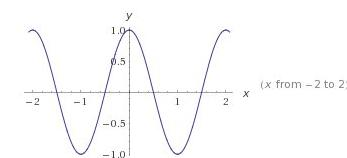
\includegraphics[scale=0.3]{cos.jpeg}
\end{center}
\end{figure}

\end{frame}

\begin{frame}
\frametitle{Bisección de f(x)=Cos($\pi$x)}

\begin{block}{}
Con el intervalo [0.2, 1.1], donde f(0.2) es positivo y f(1.1) negativo, y la fórmula del punto medio $\frac{a+b}{2}$ tenemos:$\frac{0.2+1.1}{2}=0.65$, donde f(0.65) es negativa, por lo que el cambio de signo se da en el intervalo [0.2, 0.65].
\end{block}

\begin{figure}[b]
\begin{center}
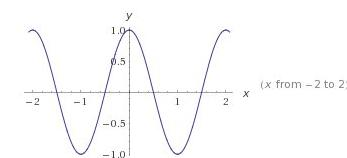
\includegraphics[scale=0.4]{cos.jpeg}
\end{center}
\end{figure}

\end{frame}

\begin{frame}
\frametitle{Bisección de f(x)=Cos($\pi$x)}

\begin{block}{}
Volvemos a repetir a operación con el nuevo intervalo, obteniendo que $\frac{0.2+0.65}{2}=0.425$, donde f(0,425) es positiva, localizandose ahora el cambio de signo en el intervalo [0.425, 0.65]. Al repetir sucesivamente obtenemos:
\begin{itemize}

  \item $\frac{0.425+0.65}{2}=0.5375$, donde f(0.5375) es negativa.
  \pause
  \item Nuevo intervalo [0.425, 0.5375].
  \pause
  \item $\frac{0.425+0.5375}{2}=0.48125$, donde f(0.48125) es positiva.
  \pause
  \item Nuevo intervalo [0.48125, 0.5375].
  \pause
  \item $\frac{0.48125+0.5375}{2}=0.509375$, donde f(0.509375) es negativa.
  \pause
  \item Nuevo intervalo [0.48125, 0.509375].
  \pause
  \item $\frac{0.48125+0.509375}{2}=0.$, donde f(0.4953125) es positiva.
  \pause
  \item Y de este modo vamos acercándonos cada vez más a 0.5, con un error que será más pequeño conforme hagamos más divisiones.
\end{itemize}
\end{block}

\end{frame}

\section{Código Python}

\begin{frame}
\frametitle{Código \textsf{Python}}
A continuación se muestra el código fuente creado en \textsf{Python} para la resolución del problema.

\begin{figure}[b]
\begin{center}
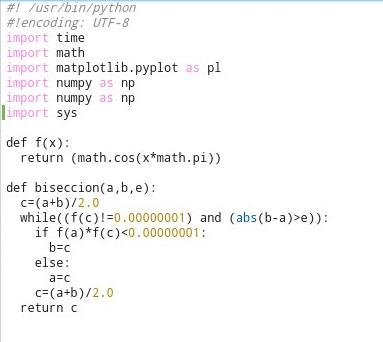
\includegraphics[scale=0.75]{python1.jpeg}
\end{center}
\end{figure}
\end{frame}

\begin{frame}
\frametitle{Código \textsf{Python}}

\begin{figure}[b]
\begin{center}
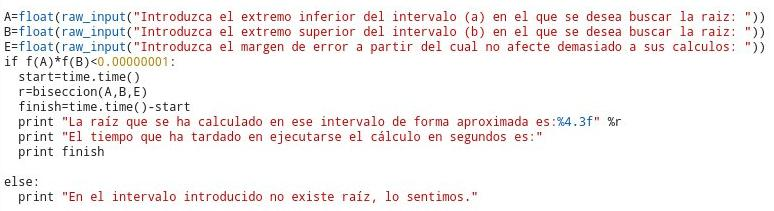
\includegraphics[scale=0.6]{python2.jpeg}
\end{center}
\end{figure}
\begin{figure}[b]
\includegraphics[width=0.2\textwidth]{images/logotipo-secundario-ULL}\\[0.25cm]
\begin{center}
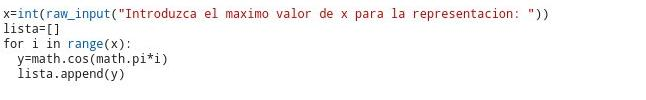
\includegraphics[scale=0.7]{python3.jpeg}
\end{center}
\end{figure}
\end{frame}

\begin{frame}
\frametitle{Código \textsf{Python}}

\begin{figure}[b]
\begin{center}
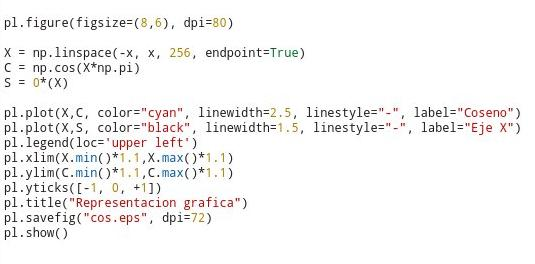
\includegraphics[scale=0.75]{python4.jpeg}
\end{center}
\end{figure}
\end{frame}

\section{Función Representada con Python}
\begin{frame}
\frametitle{Función representada con Python}

\begin{figure}[b]
\begin{center}
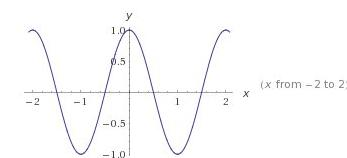
\includegraphics[scale=0.5]{cos.jpeg}
\end{center}
\end{figure}
\end{frame}

\section{La Bibliografía}

\begin{frame}
\frametitle{Bibliografía}
\begin{thebibliography}
  \beamertermplatebookbibitems
  \bibitem[Internet]{wikipedia}
  {\small $es.wikipedia.org/wiki/Método\_de\_bisección\#Algoritmo$}
  
  \beamertermplatebookbibitems
  \bibitem[Internet]{Juegos de lógica}
  {\small $www.juegosdelogica.com/numero\_\pi.htm$}
  
  \beamertermplatebookbibitems
  \bibitem[Biblioteca]{Libro}
  {\small $Análisis\_Numérico\_con\_Aplicaciones. Gerald·Wheatley. Editorial: Prentice\_Hall$}
  
  \beamertermplatebookbibitems
  \bibitem[Biblioteca]{Libro}
  {\small $Las\_Matemáticas\_del\_Cálculo\_Científico.\_David \_kincaid\_y\_Ward\_Cheney.$}
  
  \beamertermplatebookbibitems
  \bibitem[Biblioteca]{PuntoQ}
  {\small $PuntoQ:$}
  {\small$http://riunet.upv.es/handle/10251/5617$}
  {\small$http://riunet.upv.es/handle/10251/2063$}
  {\small$http://riunet.upv.es/handle/10251/5567$}
  
  \beamertermplatebookbibitems
  \bibitem[Internet]{Carmona Teaching}
  {\small $http://www.ma3.upc.edu/users/carmona/teaching/clases/08-09/trabajos/metodo\%20biseccion.pdf$}
  
  \beamertermplatebookbibitems
  \bibitem[Internet]{Github}
  {\small $Puede\_acceder\_al\_Repositorio\_online\_en:$}  
  {\small $https://github.com/alu0100833218/Equipo\_1\_A$}
  
  
\end{thebibliography}
\end{frame}

\end{document}
